\chapter{Développement d'une machine d'état pour la régulation en SISO}
\label{annexe:MachineEtatSISO}

Cette annexe présente la première machine d'état développée dans le programme. Celle-ci avait pour but d'améliorer la machine d'état déjà existante, dont l'architecture était complexe et difficilement lisible. Le comportement séquentiel défini est le suivant :

\begin{itemize}
    \item État 0 : Attente de la pression du bouton d'activation.
    \item État 1 : Montée du courant des inducteurs 1 et 2 à 3~A (afin d'éviter un démarrage à zéro).
    \item État 2 : Augmentation du courant des inducteurs 1 et 2 suivant une rampe continue (régulation de courant seule).
    \item État 3 : Basculement en régulation de position dès l'amorce du mouvement des inducteurs 1 et 2 (lévitation de la partie avant du véhicule).
    \item État 4 : Montée du courant des inducteurs 3 et 4 à 3~A.
    \item État 5 : Augmentation du courant des inducteurs 3 et 4 suivant une rampe continue (régulation de courant seule).
    \item État 6 : Basculement en régulation de position dès l'amorce du mouvement des inducteurs 3 et 4 (lévitation de la partie arrière, l'avant étant déjà sustenté).
    \item État 7 : Ajustement des gains statiques pour assurer un comportement transitoire plus doux et passage en régulation de maintien.
    \item État 8 : Arrêt de la sustentation et réinitialisation des variables.
    \item État 9 : Affichage d'un message d'erreur en cas de défaillance matérielle ou logicielle de la maquette.
\end{itemize}

Conformément à ces spécifications, l'organigramme de la \autoref{fig:MachineDEtat} a été établi :

\begin{figure}[H]
    \centering
    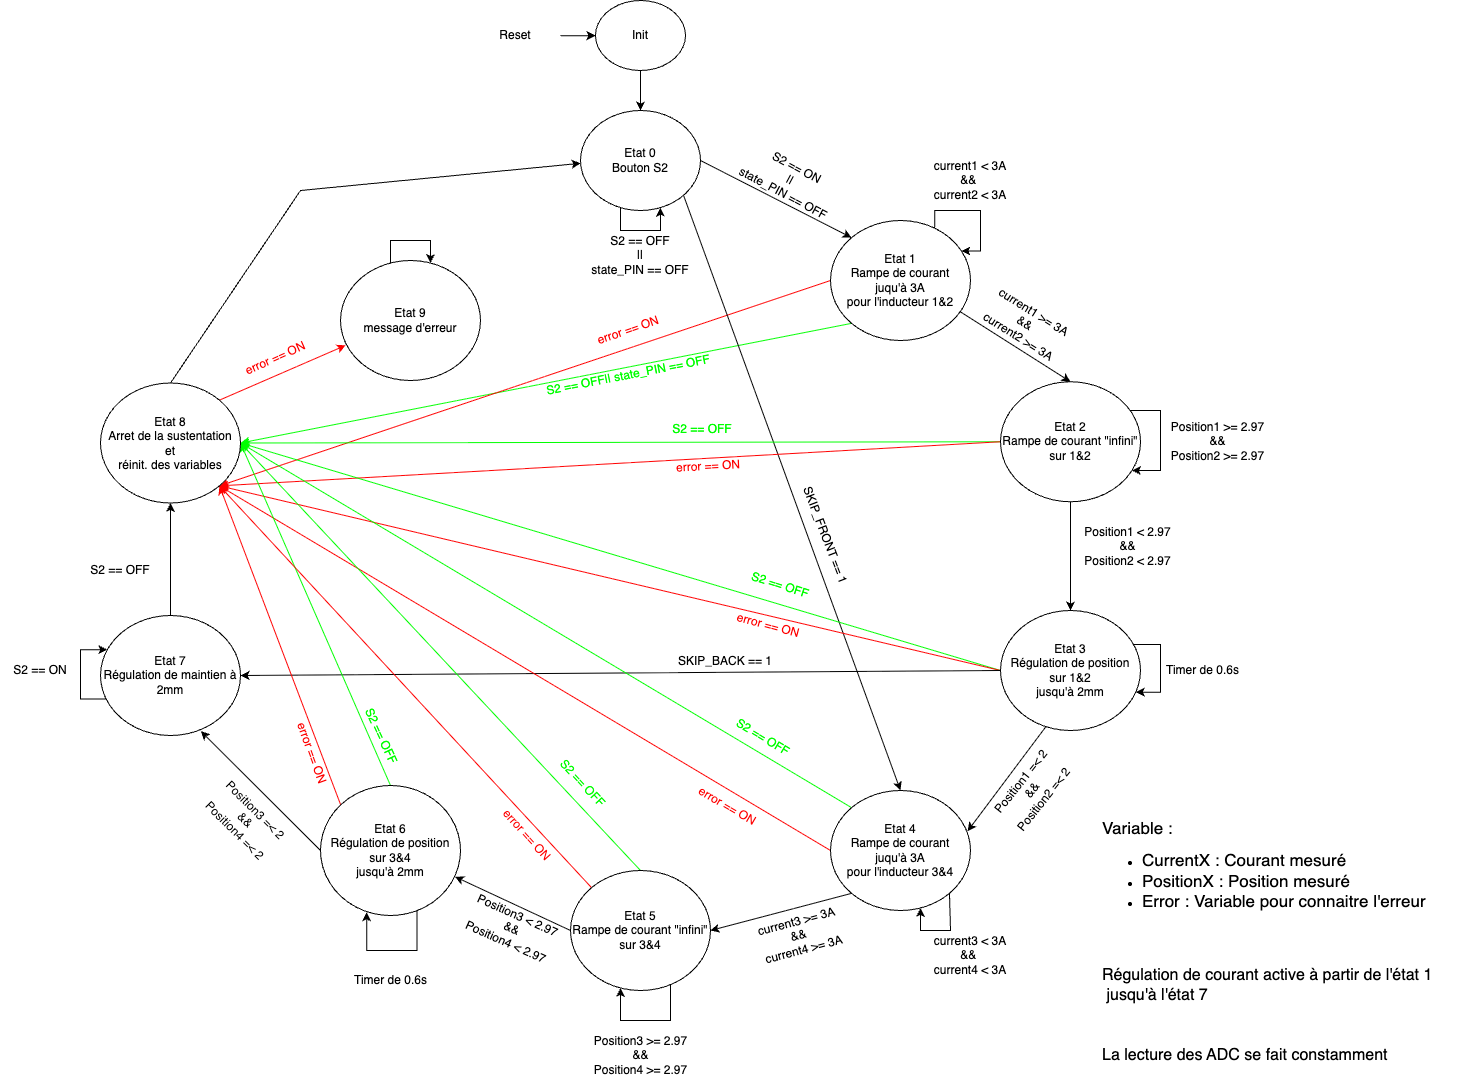
\includegraphics[width=1\linewidth]{assets/appendix/09-PremiereMachEtat/MachineDEtat.png}
    \caption{Machine d'état régissant la séquence de lévitation}
    \label{fig:MachineDEtat}
\end{figure}

Le diagramme détaillé de cette machine d'état est également disponible dans l'\autoref{an:MachineDetat}.\\

Les différents états sont implémentés dans le code source en respectant scrupuleusement la logique illustrée par la \autoref{fig:MachineDEtat}.\\

L'état 0 se définit comme une simple condition d'attente :

\begin{minted}{c}
    // State 0 :
    // Attente de la pression du bouton
    case STATE_0 :

        if(SystemOn)
        {
            GPIO_writePin(LED_D2, 0); // Allumage LED2 (Indicateur sustentation)

            // V rifie si l'on veut uniquement lever l'arrière
            state = SKIP_FRONT ? STATE_4 : STATE_1;
        }

    break;
\end{minted}

L'état 1 est programmé de la manière suivante :

\begin{minted}{c}
    // State 1 :
    // Rampe de courant sur les inducteur 1&2 jusqu'à atteindre les 3A
    case STATE_1:

        // Rampe vers 3A par pas de 0.04A
        if(ic1 < I_SP)
        {
            ic1 += TAKEOFF_CURRENT_STEP1;
        }
        else
        {
            ic1 = I_SP;
        }

        // Fixe le courant de consigne 2 par rapport à ic1
        ic2 = ic1;

        mean1 += Current1;
        mean2 += Current2;
        dt_mean++;

        if(dt_mean >= 200) // dt = 8ms
        {
            mean1 = mean1 / dt_mean;
            mean2 = mean2 / dt_mean;

            if((mean1 <= I_SP105 && mean1 >= I_SP095) && (mean2 <= I_SP105 && mean2 >= I_SP095))
            {
                // Reset des variables
                mean1 = 0;
                mean2 = 0;
                dt_mean = 0;

                // Changement d'état
                state = STATE_2;

            }
            else
            {
                // Reset des variables pour mesurer à nouveau
                mean1 = 0;
                mean2 = 0;
                dt_mean = 0;
            }
        }

        break;
\end{minted}

L'état 2 s'exécute selon la logique suivante :

\begin{minted}{c}
    // State 2 :
    // Rampe de courant "infinie" pour atteindre un courant
    // assez grand pour faire décoller l'avant
    case STATE_2:

        if(Position1 <= Position_c1_dec && Position2 <= Position_c2_dec)
        {
            // Update des variables
            Position_c1 = Position1;
            Position_c2 = Position2;

            // Changement d'état
            state = STATE_3;
        }
        else if(ic1 < 7.82f)
        {
            ic1 += TAKEOFF_CURRENT_STEP1;
        }
        else
        {
            // Fixe le courant à une valeur max
            ic1 = 7.82f;
        }

        // Fixe le courant de ic2 à ic1
        ic2 = ic1;

        break;
\end{minted}

L'état 3 est défini par le bloc de code ci-dessous :

\begin{minted}{c}
    // State 3 :
    // Activation de la régulation de position pour atteindre les 2mm
    // à l'avant
    case STATE_3:

        // Activer la régulation d'état
        if(!PosRegFlag1) PosRegFlag1 = true;

        // Set point generator (Ramp from 3mm to 2mm)
        if(Position_c1 > DELTA_N)
        {
            Position_c1 -= 2.5 * 4e-7;
        }
        else
        {
            Position_c1 = DELTA_N;
        }

        if(Position_c2 > DELTA_N)
        {
            Position_c2 -= 2.5 * 4e-7;
        }
        else
        {
            Position_c2 = DELTA_N;
        }

        // Incrémentation du timer
        i_store++;

        // Timer pour attendre un peu pour être sur que le système à bien décoller
        if(i_store == I_STORE_2E_DECOLLAGE)
        {
            // Reset de la varibale
            i_store = 0;

            if(SKIP_BACK)
            {
                state = STATE_7;
            }
            else
            {
                state = STATE_4;
            }
        }

        break;
\end{minted}

L'état 4 repose sur la structure suivante :

\begin{minted}{c}
    // State 4 :
    // Rampe de courant sur les inducteur 3&4 jusqu'à atteindre les 3A
    case STATE_4:

        // Rampe vers 3A par pas de 0.04A
        if(ic3 < I_SP)
        {
            ic3 += TAKEOFF_CURRENT_STEP1;
        }
        else
        {
            ic3 = I_SP;
        }

        // Fixe le courant de consigne 4 par rapport à ic3
        ic4 = ic3;

        mean3 += Current3;
        mean4 += Current4;
        dt_mean++;

        if(dt_mean >= 200) // dt = 8ms
        {
            mean3 = mean3 / dt_mean;
            mean4 = mean4 / dt_mean;

            if((mean3 <= I_SP105 && mean3 >= I_SP095) && (mean4 <= I_SP105 && mean4 >= I_SP095))
            {
                // Reset des variables
                mean3 = 0;
                mean4 = 0;
                dt_mean = 0;

                state = STATE_5;
            }
            else
            {
                // Reset des variables pour mesurer à nouveau
                mean3 = 0;
                mean4 = 0;
                dt_mean = 0;
            }
        }

        break;
\end{minted}

L'état 5 est implémenté selon les instructions suivantes :

\begin{minted}{c}
    // State 5 :
    // Rampe de courant "infinie" pour atteindre un courant
    // assez grand pour faire décoller l'arrière
    case STATE_5:

        if(Position3 <= Position_c3_dec && Position4 <= Position_c4_dec)
        {
            // Update des variables
            Position2_c3 = Position3;
            Position2_c4 = Position4;

            // Changement d'état
            state = STATE_6;
        }
        else if(ic3 < 7.82f)
        {
            ic3 += TAKEOFF_CURRENT_STEP1;
        }
        else
        {
            // Fixe le courant à une valeur max
            ic3 = 7.82f;
        }

        // Fixe le courant de ic4 à ic3
        ic4 = ic3;


        break;
\end{minted}

L'état 6 s'articule comme suit :

\begin{minted}{c}
    // State 6 :
    // Activation de la régulation de position pour atteindre les 2mm
    // à l'arrière
    case STATE_6:

        // Activer la régulation d'état
        if(!PosRegFlag3) PosRegFlag3 = true;

        // Set point generator (Ramp from 3mm to 2mm)
        if(Position2_c3 > DELTA_N)
        {
            Position2_c3 -= 2.5 * 4e-7;
        }
        else
        {
            Position2_c3 = DELTA_N;
        }

        if(Position2_c4 > DELTA_N)
        {
            Position2_c4 -= 2.5 * 4e-7;
        }
        else
        {
            Position2_c4 = DELTA_N;
        }

        // Incrémentation du timer
        i_store++;

        // Timer pour attendre un peu pour être sur que le système à bien décoller
        if(i_store == I_STORE_2E_DECOLLAGE)
        {
            // Reset de la varibale
            i_store = 0;

            // Changement du gain statique de l'inducteur 3
            Kr_sans_int = 0; //-1.0;

            // Changement d'état
            state = STATE_7;
        }

        break;
\end{minted}

L'état 7 est défini par les instructions de maintien :

\begin{minted}{c}
    // State 7 :
    // Régulation de maintien pour tenir la maquette en l'air
    case STATE_7:

        // Changement des variables pour une régulation plus douce
        Kr = KR_CHANGE;
        Kw = KW_CHANGE;
        Kd = KD_CHANGE;
        Kddot = KDDOT_CHANGE;

        break;

    // Default :
    // Something went wrong so let's just go to state 9 for an error
    default:
        break;
\end{minted}

Finalement, l'état 8 est défini comme une simple condition :

\begin{minted}{c}
    // State 8 :
    // Attends que le bouton soit pressé à nouveau pour éteindre la maquette
    case STATE_8:

        if(!SystemOn)
        {
            GPIO_writePin(LED_D2, 1); // Eteindre LED

            // Forcer les PWM   50%
            for(i = 0; i < NUM_OF_PWM_CHANNEL; i++)
            {
                dutyFine = ((float)(duty_cycle_table[i] * TIME_BASE_PERIOD) * INV_FACTOR);
                compCount = (dutyFine * (float32_t)(EPWM_TIMER_TBPRD << 8)) * INV_FACTOR;
                HRPWM_setCounterCompareValue(ePWM[i], HRPWM_COUNTER_COMPARE_A, compCount);
                HRPWM_setCounterCompareValue(ePWM[i], HRPWM_COUNTER_COMPARE_B, compCount);
            }

            // Reset de la machine d'état
            state = STATE_1;
            PosRegFlag1 = false;
            PosRegFlag3 = false;

            // Reset des gains d'état
            Kw = KW;
            Kd = KD;
            Kddot = KDDOT;
            Kr = KR;
            Kr_sans_int = KR_SANS_INT;

            // Reset timer
            i_store = 0;

            // 1. Reset des int grales du régulateur de courant PI et de l'anti-windup
            integral_i1 = 0.0f; ue1 = 0.0f; ic1 = 0.0f;
            integral_i2 = 0.0f; ue2 = 0.0f; ic2 = 0.0f;
            integral_i3 = 0.0f; ue3 = 0.0f; ic3 = 0.0f;
            integral_i4 = 0.0f; ue4 = 0.0f; ic4 = 0.0f;

            // 2. Reset des int grateurs de la régulation d' tat (position) et anti-windup de force
            xr1 = 0.0f; fce1 = 0.0f; ep1 = 0.0f;
            xr2 = 0.0f; fce2 = 0.0f; ep2 = 0.0f;
            xr3 = 0.0f; fce3 = 0.0f; ep3 = 0.0f;
            xr4 = 0.0f; fce4 = 0.0f; ep4 = 0.0f;

            status = SFO();
            if (status == SFO_ERROR) error();

            // Retour à l'état 0
            state = STATE_0;
        }

        break;
\end{minted}

Actuellement, l'état 9 n'est pas encore développé. À terme, son implémentation sera requise pour assurer la gestion sécurisée des erreurs et défaillances de la maquette.\\

Il est également possible de sauter l'activation de l'avant ou de l'arrière. Pour ce faire, des \texttt{\#define} ont été ajoutés en début de code, comme suit :

\begin{minted}{c}
    #define SKIP_BACK                   0
    #define SKIP_FRONT                  0
\end{minted}

La vérification d'une demande de saut de l'avant ou de l'arrière s'effectue respectivement dans l'état 0 et dans l'état 3.

Afin de permettre d'éteindre la maquette à n'importe quel moment, une simple condition a été ajoutée en amont de la machine d'état, comme suit :

\begin{minted}{c}
    if (!SystemOn && (state != STATE_0) && (state != STATE_8))
    {
        state = STATE_8;
    }
\end{minted}

Cette condition contrôle simplement que le bouton a effectivement été pressé pour demander l'arrêt (signal \texttt{SystemOn} désactivé), mais également que l'état actuel est différent de l'état 0 et de l'état 8.